%___________________________________________
% 8) Um gráfico simples y = 0,5 (reta horizontal)
%___________________________________________

\begin{figure}[H]
  \centering
  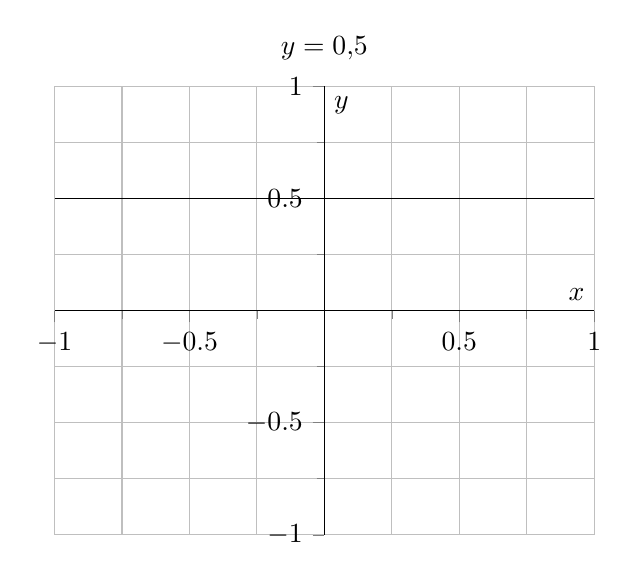
\begin{tikzpicture}
    \begin{axis}[
      xmin=-1, xmax=1,
      ymin=-1, ymax=1,
      axis x line=middle,
      axis y line=middle,
      axis line style={-},
      tick align=outside,
      grid=both,
      minor tick num=1,
      xlabel={$x$},
      ylabel={$y$},
      title={$y=0{,}5$}
    ]
      \addplot[domain=-1:1, samples=2] {0.5};
    \end{axis}
  \end{tikzpicture}
  \caption{Reta horizontal $y = 0{,}5$.}
\end{figure}